\documentclass[12pt]{article}

\usepackage[spanish]{babel}
\usepackage{hyperref}
\usepackage{graphicx}
\usepackage{listings}
\usepackage{color}
\usepackage{multicol}
\usepackage{amssymb}
\usepackage{enumitem}
\usepackage{here}
\usepackage{dsfont}
\usepackage{amsmath}
\usepackage{tipa}
\usepackage{float}
\spanishdecimal{.}

\title{Matemáticas para las Ciencias Aplicadas I}
\title{
	Cuarta Lista de Problemas \\
	\textbf{Primera  Parte} \\
	\vspace{1ex}
	\large Matemáticas para las Ciencias Aplicadas I \\
	Facultad de Ciencias, UNAM}

\date{\today}

\author{Flores Morán Julieta Melina \\ Zarco Romero José Antonio}

%% Sección 5.3: 44 y 73.
%% Sección 5.5: 28 y 37.
%% Sección 5.6: 58, 63 y 70.
%% Sección 5.8: 27.
%% Sección 5.9: 52 y 64

\begin{document}

\maketitle

%% 5.3 -----------------------------------------------------------------------------------------------------------------------------------------------------------------------------------------------------------------------------
\section{Sección 5.3 \\ Integración Por Sustitución}
% 44 -------------------------------------------------------------------------------------------------------------
\subsection{Ejercicio 44} name \\

Evaluar las integrales utilizando sustituciones apropiadas.
\[
\int \tan^3{5x}\sec^2{5x}dx
\]
Tomemos $u = \tan5x \rightarrow du = 5 \sec^{2}5xdx \rightarrow \frac{du}{5} = \sec^{2}5xdx $. \\
Sustituimos en la integral:
\[
\int u^3 \frac{du}{5}
\]
Y resolvemos normalmente:\\
\begin{align*}
  \int u^3 \frac{du}{5}
  & = \int u^3 du \frac{1}{5} \\
  & = \frac{1}{5} \int u^3 du \\
  & = \frac{1}{5} \frac {u^4}{4} + C \\
  & = \frac {u^4}{20} + C\\
\end{align*}
y regresamos a u a su valor original.
\begin{align*}
  \frac {u^4}{20} + C 
  & = \frac{\tan^45x}{20} + C
\end{align*}
% 73 -------------------------------------------------------------------------------------------------------------
\subsection{Ejercicio 73} name \\

\begin{enumerate}[label=(\alph*)]
\item Evalúe $\int \rigth[ \frac {x}{\sqrt{x^2+1}}  \left] dx$

\item Utilice una herramienta gráfica para generar algunas curvas integrales típicas de $f(x) = x / \sqrt{x^2 + 1|1}$ en el intervalo $(-5, 5)$.
  
\end{enumerate}

%% 5.5 -----------------------------------------------------------------------------------------------------------------------------------------------------------------------------------------------------------------------------
\section{Sección 5.5 \\ La Integral Definida}
% 28 -------------------------------------------------------------------------------------------------------------
\subsection{Ejercicio 28} name \\

Utilice el Teorema 5.5.4 y fórmulas apropiadas de geometría para evaluar las integrales. \\

\[
\int_{-3}^{0} \left(2+\sqrt{9-x^2} \right)dx
\]
Siguiendo el teorema 5.5.4, esta integral equivale a : \\
\[
\int_{-3}^{0}  2 dx +  \int_{-3}^{0} \sqrt{9-x^2} \right)dx
\]
Procedamos a evaluar la primera integral $\int_{-3}^{0} 2 dx$ donde podemos ver la función $y=2$ que es una línea recta horizontal, por lo que el área formada con el eje x en el intervalo de 0 a -3 es un rectángulo de altura 2 y de base $|-3| = 3$, así que el área es $3 \cdot 2$ y entonces
\[
\int_{-3}^{0}  2 dx  = 6
\]
Para la segunda integral  $ \int_{-3}^{0} \sqrt{9-x^2}\right)dx$. Tenemos que  $y = \sqrt{9-x^2}  $ delimita la región de un cuarto de un circulo donde $r^2 = 9$ y por lo tanto su radio es de 3. \\ Considerando la formular del área de un circulo tenemos que el área de la cuarta parte es $\frac{1}{4} \pi (3)^2$, por lo tanto.
\[
 \int_{-3}^{0} \sqrt{9-x^2} \right)dx  = \frac{9\pi}{4}
 \]
 Por lo tanto el resultado de la suma de ambas sería: \\
 \[
\int_{-3}^{0}  2 dx +  \int_{-3}^{0} \sqrt{9-x^2}\right)dx = 6 + \frac{9\pi}{4} 
\]
Lo que resuelve la integral dada.
\[
\int_{-3}^{0} \left(2+\sqrt{9-x^2}\right)dx  = 6 + \frac{9\pi}{4} 
\]
% 37 -------------------------------------------------------------------------------------------------------------
\subsection{Ejercicio 37} name \\

Evaluar las integrales completando el cuadrado y aplicando fórmulas apropiadas de geometría.
\[
\int_{0}^{10} \sqrt{10x-x^2}dx
\]

%% 5.6 -----------------------------------------------------------------------------------------------------------------------------------------------------------------------------------------------------------------------------
\section{Sección 5.6 \\ El Teorema Fundamental Del Cálculo}
% 58 -------------------------------------------------------------------------------------------------------------
\subsection{Ejercicio 58} name \\

Defina $F (x)$ por
\[
F(x)=\int_{\pi/4}^{x} \cos{2t} dt
\]
\begin{enumerate}[label=(\alph*)]
\item Utilice la parte 2 del teorema fundamental del cálculo para encontrar $F'(x)$. \\
  La parte 2 del teorema fundamental del cálculo nos dice que $\frac{d}{dx}\left[ \int_{a}^{x} f(t)dt \right] = f(x)$. En este caso el integrando es una función continua, entonces $f(x) = cos2x$. Por lo tanto $F'(x) = \cos{2x}$
\item Verifique el resultado del inciso (a) integrando primero y luego diferenciando. \\
Podemos resolver la integral mediante un cambio de variable. $u= 2t \rightarrow du = 2dt  \rightarrow dt = \frac{du}{2}$\\
\begin{align*}
  F(x)=
  & = \int_{\pi/4}^{x} \cos{2t} dt \\
  & = \int_{\pi/4}^{x} \cos{u} \frac{du}{2}\\
  & = \frac{1}{2} \int_{\pi/4}^{x} \cos{u} du \\
  & = \frac{1}{2} \sen u \Bigg|_{\pi/4}^{x} \\
  & = \frac{1}{2} \sen 2t \Bigg|_{\pi/4}^{x} \\
  & = \frac{1}{2} \left[  \sen 2x - \sen 2\frac{\pi}{4} \right] \\
  & = \frac{1}{2} \left[  \sen 2x - 1 \right]\\
  & = \frac{1}{2}  \sen 2x - \frac{1}{2}  
\end{align*}
Y ahora podemos derivar $F(x)$.
\begin{align*}
  F'(x)=
  & = \frac{d}{dx} \left[ \frac{1}{2}  \sen 2x - \frac{1}{2} \right]  \\
  & = \frac{1}{2}  \cos 2x \cdot 2 \\
  & = \cos 2x  \\
\end{align*}
\end{enumerate}

% 63 -------------------------------------------------------------------------------------------------------------
\subsection{Ejercicio 63} name \\

Sea $F(x)=\int_{4}^{x} \sqrt{t^2+9}dt$. Encuentre
\begin{enumerate}[label=(\alph*)]
\item $F(4)$.
  
\item $F'(4)$.
  
\item $F''(4)$.
  
\end{enumerate}

% 70 -------------------------------------------------------------------------------------------------------------
\subsection{Ejercicio 70} name \\

Un ingeniero de tránsito monitorea la velocidad a la que los automóviles ingresan a la carretera principal durante la hora pico de la tarde. De sus datos estima que entre las 16:30 horas. y 17:30 p.m. la tasa  $R(t)$ a la que los automóviles ingresan a la carretera está dada por la fórmula $R(t) = 100 (1$ - $0.0001t^2 )$ automóviles por minuto, donde $t$ es el tiempo (en minutos) desde las 4:30 p.m.
\begin{enumerate}[label=(\alph*)]
\item ¿Cuándo ocurre el flujo máximo de tráfico hacia la carretera?\\
El flujo máximo de autos ocurre cuando R(t) alcanza su valor máximo. Esto es cuando $t=0$ ya que el factor  $(1 - 0.0001t^2 ) $ sería 1 y el flujo de autos es 100, esto ocurre a las 16:30.
\item Estime el número de automóviles que entran a la carretera durante la hora pico.\\
  Para avaluar el número de autos que entran, debemos evaluar la suma de las tasas de entrada en cada momento de esa hora transcurrida entre $16:30$ y $17:30$, es decir, en un periodo de 0 a 60 minutos ya que $t=0$ equivale a $16:30$ y $t=60$ a $17:30$.Entonces evaluemos:\\
\begin{align*}
  \int_0^{60} \rigth[ 100 (1- 0.0001t^2) dt \left]
  & = 100 \rigth[ \int_0^{60}  (1- 0.0001t^2) dt \left]\\
  & =  100 \rigth[ \int_0^{60}dt - 0.0001 \int_0^{60} t^2 dt \left]\\
  & =  100 \rigth[ \int_0^{60}dt - 0.0001 \int_0^{60} t^2 dt \left]\\
  & =  100 \rigth[ t \Bigg|_0 ^{60} - 0.0001 \frac {t^3}{3} \Bigg|_0 ^{60} \left]\\
  & =  100 \rigth[ (60-0) - 0.0001 ( \frac {60^3}{3}  -  \frac {0^3}{3}) \left]\\
  & =  100 \rigth[ 60 - 0.0001 ( 72000 ) \left]\\
  & =  100 \cdot 52.8\\
  & =   5280
\end{align*}
Así que el número de coches entrados a la carretera en la hora pico fue de 5280.
\end{enumerate}

%% 5.8 -----------------------------------------------------------------------------------------------------------------------------------------------------------------------------------------------------------------------------
\section{Sección 5.8 \\ Valor Promedio De Una Función Y Sus Aplicaciones}
% 27 -------------------------------------------------------------------------------------------------------------
\subsection{Ejercicio 27} name \\

Un ingeniero de tránsito monitorea la velocidad a la que los automóviles ingresan a la carretera principal durante la hora pico de la tarde. De sus datos estima que entre las 16.30 horas. y 5:30 p.m. la velocidad $R(t)$ a la que los automóviles ingresan a la carretera está dada por la fórmula $R(t) = 100(1 − 0.0001t^2)$ automóviles por minuto, donde $t$ es el tiempo (en minutos) desde las 4:30 p.m. Encuentre la velocidad promedio, en automóviles por minuto, a la que los automóviles ingresan a la carretera durante la primera media hora de la hora pico.

%% 5.9 -----------------------------------------------------------------------------------------------------------------------------------------------------------------------------------------------------------------------------
\section{Sección 5.9 \\ Evaluación De Integrales Definidas Por Sustitución}
% 52 -------------------------------------------------------------------------------------------------------------
\subsection{Ejercicio 52} name \\

\begin{enumerate}[label=(\alph*)]
\item Utilice un CAS para encontrar el valor exacto de la integral
  \[
  \int_{-\pi/4}^{\pi/4} \tan^4{x} dx
  \]
\item Confirme el valor exacto mediante cálculo manual. [\textit{Sugerencia}: Utilice la identidad $1 + \tan^2{x}=\sec^2{x}$.]\\
  Utilizando la identidad reescrita como $\tan^2{x}=\sec^2{x}-1$  podemos reescribir la integral de la siguiente forma:
  \begin{align*}
    \int_{-\pi/4}^{\pi/4} \tan^4{x} dx
    & = \int_{-\pi/4}^{\pi/4} \rigth[ \tan^2{x} \cdot (\sec^2{x}-1) \left]dx \\
    & = \int_{-\pi/4}^{\pi/4} [\tan^2{x} \cdot \sec^2{x} -  \tan^2{x} ] dx \\
    & = \int_{-\pi/4}^{\pi/4} [\tan^2{x} \cdot \sec^2{x} -  \tan^2{x} ] dx \\
    & = \int_{-\pi/4}^{\pi/4} \tan^2{x} \cdot \sec^2{x} dx - \int_{-\pi/4}^{\pi/4}   \tan^2{x}  dx \\
  \end{align*}
\end{enumerate}
Podemos usar sustitución para la primera integral, donde $u= tanx \rightarrow du=sec^{2}x dx$.\\
  \begin{align*}
    \int_{-\pi/4}^{\pi/4} \tan^2{x} \cdot \sec^2{x} dx
    & = \int_{-\pi/4}^{\pi/4} u^2 \cdot du \\
    & = \frac{u^{3}}{3} \Bigg|_{-\pi/4}^{\pi/4} \\
    & = \frac{tan^{3}x}{3} \Bigg|_{-\pi/4}^{\pi/4} \\
  \end{align*}
  Y la fórmula dada en el formulario para la segunda.
    \begin{align*}
      \int_{-\pi/4}^{\pi/4}   \tan^2{x}  dx
      & = tanx - x  \Bigg|_{-\pi/4}^{\pi/4}
    \end{align*}
    Así podemos reescribir:
      \begin{align*}
        \int_{-\pi/4}^{\pi/4} \tan^2{x} \cdot \sec^2{x} dx - \int_{-\pi/4}^{\pi/4}   \tan^2{x}  dx 
        & = \left( \frac{tan^{3}x}{3} -[ tanx - x] \right)  \Bigg|_{-\pi/4}^{\pi/4}\\
        & =  \left( \frac{tan^{3}x}{3} - tanx + x \right) \Bigg|_{-\pi/4}^{\pi/4}\\
        & =  \frac{tan^{3}(\frac{\pi}{4})}{3} - tan(\frac{\pi}{4}) + \frac{\pi}{4}  - \left[  \frac{tan^{3}(\frac{-\pi}{4})}{3} - tan(\frac{-\pi}{4}) + \frac{-\pi}{4} \right] \\
        & =  \frac{tan^{3}(\frac{\pi}{4})}{3} - tan(\frac{\pi}{4}) + \frac{\pi}{4}  -   \frac{tan^{3}(\frac{-\pi}{4})}{3} + tan(\frac{-\pi}{4}) + \frac{\pi}{4}  \\
        & =  \frac{1}{3} - 1 + \frac{\pi}{4}  +   \frac{1} {3} - 1 + \frac{\pi}{4}  \\
        & =  \frac{2}{3} - 2 + \frac{\pi}{2}   \\
        & =  -\frac{4}{3} + \frac{\pi}{2}   \\
      \end{align*}
Por lo tanto el valor exacto es $-\frac{4}{3} + \frac{\pi}{2} \approx 0.2374629935 $.
% 64 -------------------------------------------------------------------------------------------------------------
\subsection{Ejercicio 64} name \\

\begin{figure}[H]
\centering
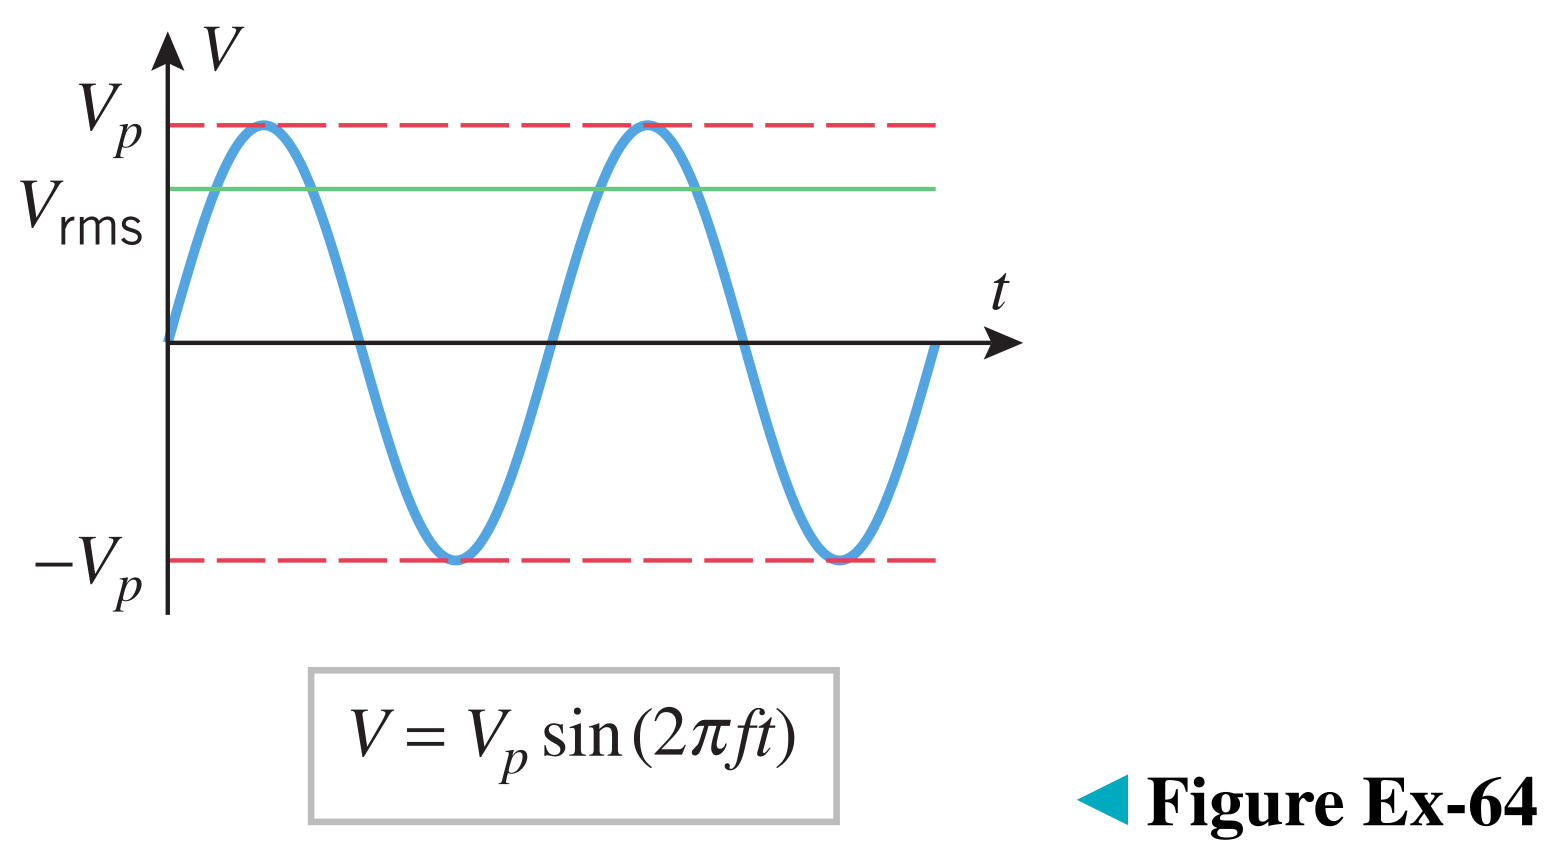
\includegraphics[width=0.7\textwidth]{../img/img_Lista4/1_64.png}
\end{figure}

La electricidad se suministra a los hogares en forma de \textbf{\textit{corriente alterna}}, lo que significa que el voltaje tiene una forma de onda sinusoidal descrita por una ecuación de la forma
\[
V = V_p \sin{(2\pi ft)}
\]
(ver la figura adjunta). En esta ecuación, $V_p$ se llama \textbf{\textit{voltaje máximo}} o \textbf{\textit{amplitud}} de la corriente, $f$ se llama \textbf{\textitfrecuencia}} y $1/f$ se llama \textbf{\textit{período}}. Los voltajes $V$ y $V_p$ se miden en voltios ($V$), el tiempo $t$ se mide en segundos ($s$) y la frecuencia se mide en hercios ($Hz$). ($1 Hz = 1$ ciclo por segundo; un \textbf{\textit{ciclo}} es el término eléctrico para un período de la forma de onda). La mayoría de los voltímetros de corriente alterna leen lo que se llama \textbf{\textit{rms}} o \textbf{\textit{valor cuadrático medio}} de $V$. Por definición, ésta es la raíz cuadrada del valor promedio de $V^2$ durante un período.
\begin{enumerate}[label=(\alph*)]
\item Demuestre que
  \[
  V_{rms}=\frac{V_p}{\sqrt{2}}
  \]
    [\textit{Sugerencia}: Calcule el promedio durante el ciclo de $t= 0$ a $t = 1/f$ y use la identidad $\sin^2{\theta}= \frac{1}{2}(1-\cos{2\theta})$ para ayudar a evaluar la integral.]
  
\item En Estados Unidos, los enchufes eléctricos suministran corriente alterna con un voltaje $rms$ de $120 V$ a una frecuencia de $60 Hz$. ¿Cuál es el voltaje máximo en tal toma corriente?

\end{document}
